\documentclass[conference]{IEEEtran}

% ---------------------------------------------------------------------------
% Packages (all available on Overleaf's standard TeX Live image)
% ---------------------------------------------------------------------------
\usepackage{cite}
\usepackage{amsmath,amssymb,amsfonts}
\usepackage{graphicx}
\usepackage{booktabs}
\usepackage{multirow}
\usepackage{algorithm}
\usepackage{algpseudocode}
\usepackage{xcolor}
\usepackage{url}
\usepackage{tikz}
\usetikzlibrary{positioning,arrows.meta,decorations.pathreplacing,calc}
\usepackage{pgfplots}
\pgfplotsset{compat=1.18}

\def\BibTeX{{\rm B\kern-.05em{\sc i\kern-.025em b}\kern-.08em
    T\kern-.1667em\lower.7ex\hbox{E}\kern-.125emX}}

\begin{document}

\title{Query-Driven Localization of On-Screen Spoken Dialogue in Video Using Speaker-Consistent Active Speaker Verification}

% Replace the placeholders below with the real author details.
\author{
\IEEEauthorblockN{Author Name One}
\IEEEauthorblockA{\textit{Department of Computer Science and Engineering} \\
\textit{Institution Name}\\
City, Country \\
email@institution.edu}
\and
\IEEEauthorblockN{Author Name Two}
\IEEEauthorblockA{\textit{Department of Computer Science and Engineering} \\
\textit{Institution Name}\\
City, Country \\
email@institution.edu}
}

\maketitle

% ---------------------------------------------------------------------------
\begin{abstract}
Searching a video for a line of dialogue is usually treated as text retrieval over subtitles or an automatic transcript. Such a search finds the moment a line is heard, but it cannot say whether the person saying it is visible. For editors, archivists and fact-checkers that difference matters, because a line delivered to camera and the same line in voice-over are different pieces of evidence. We present a pipeline that takes a video URL and an optional target line and returns the first frame in which the line is spoken by a visible, actively speaking person, along with its timestamp, recognized text, the frame image and a confidence score broken down by source. The method combines word-level speech recognition, speaker diarization and audio-visual active speaker detection. Its frame-selection rule accepts a frame only when the speaking face belongs to the diarized speaker of the queried words, the speaking run lasts a minimum duration expressed in milliseconds, and the run does not cross a shot boundary. Candidate windows are located in the transcript first and verified visually afterwards, so a targeted query on a 610\,s test video sent only 0.7\% of the footage for visual analysis. Without a query, the same pipeline sorts every utterance into on-screen, ambiguous and off-camera groups; on the test video it ruled 17 of 31 utterances off camera, including an entire internal-monologue scene. We also report integration findings, such as an undocumented minimum clip length in the hosted detector, that affect any system built from the same components.
\end{abstract}

\begin{IEEEkeywords}
active speaker detection, speaker diarization, automatic speech recognition, audio-visual verification, dialogue localization, video retrieval
\end{IEEEkeywords}

% ---------------------------------------------------------------------------
\section{Introduction}
\label{sec:intro}

A request such as ``find where the character says \emph{my mind rebels at stagnation}'' looks like a search problem, and most tools treat it as one. Subtitle files, platform captions and automatic transcripts can all be searched for a phrase, and recognizers such as Whisper~\cite{radford2023whisper} make a transcript cheap to obtain for almost any video. What these tools return, however, is the time at which a line is \emph{heard}. They say nothing about whether the person producing it is in the shot. In edited material the two often diverge: a line may be delivered over a reaction shot of another character, replayed in a flashback, narrated as internal monologue, or reused in a trailer over unrelated footage.

For several kinds of users the visible delivery is exactly what is being searched for. An assistant editor looking for the take in which an actor says a line on camera has no use for a voice-over occurrence. An archivist clearing a clip for licensing needs to know who is visibly speaking. A fact-checker verifying a quotation wants footage of the speaker saying it, not an audio track laid over unrelated shots. In all three cases a text hit is only a candidate, and someone still has to watch the footage to confirm it.

This paper automates that confirmation step. Given a video URL and, optionally, a target line, the system returns the first frame in which the line is spoken by a person who is visible and actively speaking. The output includes the timestamp, the frame index, the recognized text, the frame image and a confidence value that is broken down into its sources. When no line is given, the system examines every utterance and reports which ones are delivered on screen, which are uncertain and which are spoken off camera.

No single pretrained model answers this question. Active speaker detection (ASD) models~\cite{roth2020ava,min2022spell,liao2023lightasd,wang2024loconet} score whether a visible face is talking, but they have no notion of a query. Speech recognition and diarization~\cite{bain2023whisperx,bredin2023pyannote} recover what was said and by whom, but not who was visible. Recent character-aware subtitling systems~\cite{korbar2024llr,huh2024context} attach names to speech, yet they do not report whether, or at which frame, the speaker appears. We therefore compose these components and concentrate on the parts the composition itself demands: deciding where to look, checking that the face found speaking belongs to the speaker of the queried words, and reducing per-frame detector output to one defensible frame.

The contributions of this work are as follows.
\begin{itemize}
\item A formulation of on-screen dialogue localization as a search for the earliest frame that satisfies a speaker-consistent, temporally persistent speaking predicate, and a \emph{localize-then-verify} pipeline whose visual cost depends on the number of transcript matches rather than on video length.
\item A frame-selection rule with four explicit conditions (speaker agreement, a minimum speaking duration defined in milliseconds, no shot-cut crossing, and frame contiguity), each of which reports its own failure reason.
\item An interpretable confidence score that drops, rather than credits, the text-match term when no query exists, so that both operating modes share one scale, together with a three-way outcome (\textit{success}, \textit{ambiguous}, \textit{not on screen}) carrying machine-readable reasons.
\item Measured integration findings, including an undocumented minimum clip length in the hosted ASD service and the effect of request ordering on its output, and an open implementation available as a command-line tool, an HTTP API and a web interface.
\end{itemize}

Section~\ref{sec:related} reviews related work, Section~\ref{sec:problem} formalizes the task and Section~\ref{sec:method} describes the method. Section~\ref{sec:impl} covers the implementation, Sections~\ref{sec:setup} and~\ref{sec:results} the evaluation, and Section~\ref{sec:discussion} the limitations.

% ---------------------------------------------------------------------------
\section{Related Work}
\label{sec:related}

\subsection{Active Speaker Detection}
The AVA-ActiveSpeaker benchmark~\cite{roth2020ava} framed ASD as per-face, per-frame classification on movie footage, and most later work is measured on it. TalkNet~\cite{tao2021talknet} showed the value of long temporal context. SPELL~\cite{min2022spell} represents each person in each frame as a graph node and treats ASD as node classification, reaching 94.2\% mAP with a visual encoder of about 0.7~GFLOPs. Light-ASD~\cite{liao2023lightasd} reaches 94.1\% with 1.0\,M parameters by separating 2-D and 3-D convolutions and modelling cross-modal context with a GRU. Its journal extension, LR-ASD~\cite{liao2025lrasd}, reports 94.5\% with 0.84\,M parameters and better cross-dataset transfer. LoCoNet~\cite{wang2024loconet} interleaves long-term intra-speaker and short-term inter-speaker modelling and reaches 95.2\%, gaining most in multi-speaker scenes; the TalkNCE contrastive loss~\cite{jung2023talknce} lifts it to 95.5\%. Recent preprints push AVA results further, either by decoupling temporal and social reasoning~\cite{xiao2025d2stream} or by fusing audio, face and mouth streams with modality dropout~\cite{wang2026roam}. One of them adds enrolled speaker embeddings so that a registered speaker can be recognized even when off screen~\cite{wang2026beyond}. UniTalk~\cite{nguyen2026unitalk} warns that AVA, built mostly from older films, overstates real-world accuracy: models close to saturation on AVA fall clearly short on modern, noisy and crowded footage. Lip-synchronization models~\cite{chung2016syncnet,afouras2020lwtnet,iashin2024synchformer} address a closely related question, whether audio and mouth motion agree, and several systems use them to find the talking face.

These detectors produce strong frame-level scores, but they take pre-tracked faces as input and answer only ``is this face speaking now?''. None accepts a line of dialogue as a query or decides at which frame that line begins to be spoken on camera.

\subsection{Speech Recognition and Diarization}
Whisper~\cite{radford2023whisper} provides robust zero-shot transcription, but its native timestamps are coarse. WhisperX~\cite{bain2023whisperx} adds voice-activity segmentation, batched decoding and phoneme-level forced alignment; it raises word-segmentation precision on AMI from 78.9 to 84.1 and runs 11.8 times faster. The neural diarization models in pyannote.audio~\cite{bredin2023pyannote,plaquet2023powerset} answer ``who spoke when'' with anonymous labels. Both families work on audio alone, so even a transcript with perfect speaker labels cannot separate a voice-over from an on-camera line.

\subsection{Audio-Visual Diarization and Subtitling}
AVA-AVD~\cite{xu2022avaavd} introduced a 29-hour audio-visual diarization set drawn from 117 films, together with the AVR-Net model, which reaches 20.57\% diarization error rate (DER) with oracle voice activity. Its authors single out off-screen speakers as a central difficulty. Korbar \textit{et al.}~\cite{korbar2024llr} build per-character voice exemplars from audio-visual evidence and use them to label every speech segment of a television episode. Huh and Zisserman~\cite{huh2024context}, whose system we take as the base work for this study, extend that pipeline. They use WhisperX transcription, LWTNet synchrony~\cite{afouras2020lwtnet} to find the talking face, CLIP-based character recognition, and a large language model that assigns short segments from dialogue context. On three sitcoms they lower DER from 26.4--28.0\% to 20.3--25.7\%.

That line of work is the closest to ours in its components, but it answers a different question. Its output is a character name for each speech segment. Off-screen speech is attributed to a character by voice, which suits subtitles but removes precisely the distinction this paper needs. It also assumes a cast list and gallery images for each show, and it processes whole episodes. Table~\ref{tab:compare} summarizes the differences.

\begin{table}[t]
\centering
\caption{Capabilities of related systems and of the proposed pipeline}
\label{tab:compare}
\resizebox{\columnwidth}{!}{%
\begin{tabular}{lcccccc}
\toprule
Method & Tr. & Spk. & Vis. & Query & Frame & Off \\
\midrule
ASD models~\cite{min2022spell,liao2023lightasd,wang2024loconet,liao2025lrasd} & -- & -- & \checkmark & -- & $\circ$ & -- \\
ROAM-ASD-CR~\cite{wang2026beyond} & -- & $\circ$ & \checkmark & -- & $\circ$ & $\circ$ \\
WhisperX~\cite{bain2023whisperx} & \checkmark & $\circ$ & -- & -- & -- & -- \\
AVR-Net~\cite{xu2022avaavd} & -- & \checkmark & \checkmark & -- & -- & -- \\
LLR~\cite{korbar2024llr} & \checkmark & \checkmark & \checkmark & -- & -- & -- \\
Huh and Zisserman~\cite{huh2024context} & \checkmark & \checkmark & \checkmark & -- & -- & -- \\
\midrule
This work & \checkmark & \checkmark & \checkmark & \checkmark & \checkmark & \checkmark \\
\bottomrule
\end{tabular}}

\vspace{3pt}
\parbox{\columnwidth}{\scriptsize Tr.: produces a transcript; Spk.: speaker attribution; Vis.: visual verification; Query: accepts a text query; Frame: returns one exact frame for a line; Off: explicit off-screen verdict per line; $\circ$: partial.}
\end{table}

% ---------------------------------------------------------------------------
\section{Problem Formulation}
\label{sec:problem}

Let a video consist of frames $f\in\{0,\dots,F-1\}$ shown at a constant rate of $r$ frames per second, so that frame $f$ is presented at
\begin{equation}
t(f)=f/r .
\label{eq:cfr}
\end{equation}
Equation~\eqref{eq:cfr} holds only for constant-frame-rate (CFR) media. For variable-frame-rate sources the mapping between frame index and time is not linear, which is why the method normalizes every input before any timing computation.

The audio yields a word sequence $\mathcal{W}=(w_1,\dots,w_N)$. Each word has an interval $[s_i,e_i]$, a recognizer probability $\pi_i$ and, after diarization, a speaker label $\sigma(w_i)$ that may be undefined. A query $q$ matches a contiguous span of words whose majority speaker is $\sigma_q$.

For each frame, an ASD model reports a set of faces $\Phi(f)$. Each face $\phi$ carries a speaking flag $a(\phi)\in\{0,1\}$, a detection confidence $c(\phi)$ and, when the model receives diarization, the speaker label $\lambda(\phi)$ it associates with that face. The on-screen predicate for the query speaker is
\begin{equation}
S_q(f)=\exists\,\phi\in\Phi(f):\ a(\phi)=1\ \wedge\ \lambda(\phi)=\sigma_q .
\label{eq:pred}
\end{equation}
Let $k$ be a minimum run length (Section~\ref{sec:select}) and $\mathcal{K}$ the set of frames that begin a new shot. The answer is the earliest frame inside a candidate window $\mathcal{F}_q$ that opens a qualifying run:
\begin{multline}
f^\ast=\min\bigl\{f\in\mathcal{F}_q : S_q(f+m)\ \ \forall m\in[0,k), \\
\{f+1,\dots,f+k-1\}\cap\mathcal{K}=\emptyset\bigr\}.
\label{eq:target}
\end{multline}
If no such frame exists in any candidate window, the line is reported as \emph{not on screen}; if no transcript span matches $q$, it is reported as \emph{not found}. These two negative answers are kept apart because they send the user in different directions. Without a query, \eqref{eq:target} is evaluated separately for every speech segment, with $\sigma_q$ replaced by the speaker of that segment.

% ---------------------------------------------------------------------------
\section{Proposed Method}
\label{sec:method}

Fig.~\ref{fig:pipeline} shows the pipeline. Audio processing runs once per video; visual verification runs once per candidate window.

\begin{figure*}[t]
\centering
\resizebox{\textwidth}{!}{%
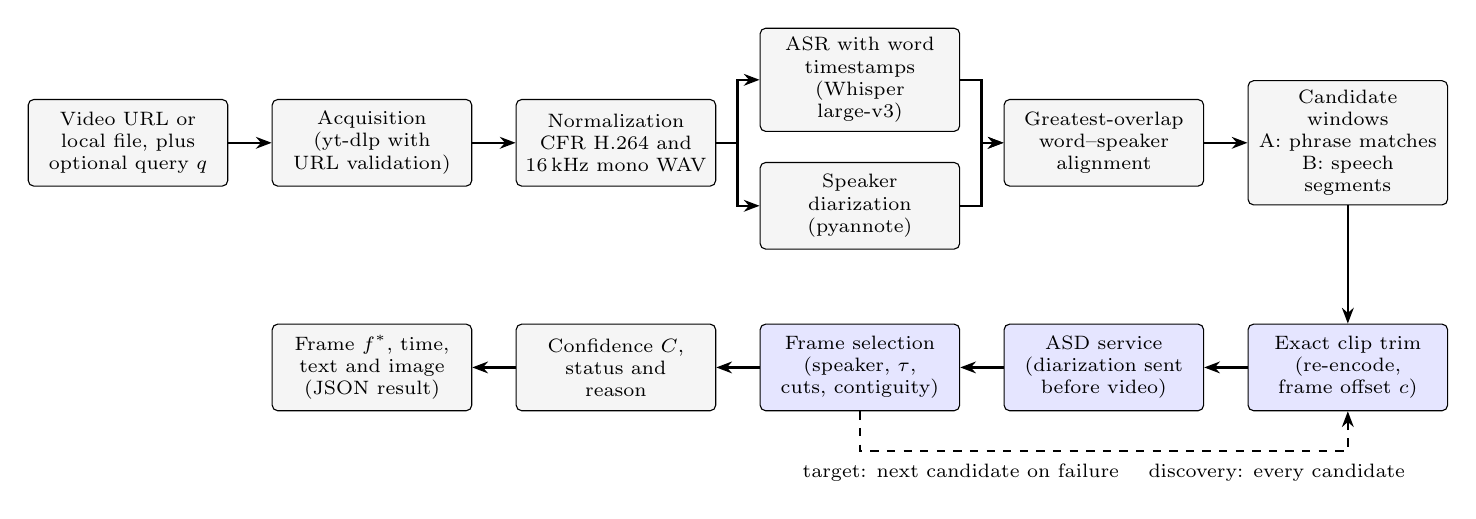
\begin{tikzpicture}[
  blk/.style={draw, rounded corners=2pt, align=center, minimum height=1.1cm, text width=2.3cm, font=\scriptsize, fill=gray!8},
  hl/.style={blk, fill=blue!10},
  arr/.style={-{Stealth[length=2mm]}, thick},
  node distance=0.55cm
]
\node[blk] (in) {Video URL or\\local file, plus\\optional query $q$};
\node[blk, right=of in] (acq) {Acquisition\\(yt-dlp with\\URL validation)};
\node[blk, right=of acq] (norm) {Normalization\\CFR H.264 and\\16\,kHz mono WAV};
\node[blk, right=of norm, yshift=0.8cm] (asr) {ASR with word\\timestamps\\(Whisper large-v3)};
\node[blk, right=of norm, yshift=-0.8cm] (dia) {Speaker\\diarization\\(pyannote)};
\node[blk, right=of asr, yshift=-0.8cm] (aln) {Greatest-overlap\\word--speaker\\alignment};
\node[blk, right=of aln] (cand) {Candidate windows\\A: phrase matches\\B: speech segments};
\node[hl, below=1.5cm of cand] (clip) {Exact clip trim\\(re-encode,\\frame offset $c$)};
\node[hl, left=of clip] (asd) {ASD service\\(diarization sent\\before video)};
\node[hl, left=of asd] (sel) {Frame selection\\(speaker, $\tau$,\\cuts, contiguity)};
\node[blk, left=of sel] (conf) {Confidence $C$,\\status and\\reason};
\node[blk, left=of conf] (out) {Frame $f^\ast$, time,\\text and image\\(JSON result)};
\draw[arr] (in) -- (acq);
\draw[arr] (acq) -- (norm);
\draw[arr] (norm.east) -- ++(0.27,0) |- (asr.west);
\draw[arr] (norm.east) -- ++(0.27,0) |- (dia.west);
\draw[arr] (asr.east) -- ++(0.27,0) |- (aln.west);
\draw[arr] (dia.east) -- ++(0.27,0) |- (aln.west);
\draw[arr] (aln) -- (cand);
\draw[arr] (cand) -- (clip);
\draw[arr] (clip) -- (asd);
\draw[arr] (asd) -- (sel);
\draw[arr] (sel) -- (conf);
\draw[arr] (conf) -- (out);
\draw[arr, dashed] (sel.south) -- ++(0,-0.5) -| (clip.south);
\node[font=\scriptsize, anchor=north] at ([yshift=-0.55cm]asd.south) {target: next candidate on failure \quad discovery: every candidate};
\end{tikzpicture}}
\caption{Overview of the proposed pipeline. The upper row runs once per video and its outputs are cached. The shaded lower row runs once per candidate window; in target mode it stops at the first window that verifies.}
\label{fig:pipeline}
\end{figure*}

\subsection{Acquisition and Normalization}
Remote URLs are fetched with yt-dlp~\cite{ytdlp} after a validation step that rejects non-HTTP schemes and hosts that resolve to private addresses. A local file path is accepted as a fallback when a site refuses automated download. FFmpeg~\cite{ffmpeg} then produces two artefacts in one decoding pass. The first is an H.264 video forced to a constant frame rate at the source's measured average rate, limited to 1080 lines and written with its index atom at the start of the file. The second is a 16\,kHz mono PCM track for the audio models. The output is probed again rather than trusted, and the measured rate $r$ is the value used in every later conversion. Forcing CFR is what makes the frame index returned to the user and the timestamp printed beside it agree by construction.

\subsection{Transcription, Diarization and Alignment}
Speech is transcribed with Whisper large-v3 through the faster-whisper runtime~\cite{fasterwhisper}, with word timestamps enabled. Decoding is made deterministic. Temperature is fixed at zero, which disables the default fallback ladder that resamples low-confidence segments; conditioning on previous text is switched off; and the beam width is fixed at five. Diarization uses the pyannote community-1 pipeline~\cite{bredin2023pyannote}. Turns shorter than 0.25\,s are discarded: on our test material 24\% of raw turns fell below this length, the shortest lasting 17\,ms, and keeping them split single sentences between two speakers.

The two timelines are joined by giving each word the speaker of the turn it overlaps most,
\begin{equation}
\sigma(w_i)=\operatorname*{arg\,max}_{u\in\mathcal{U}} \bigl|[s_i,e_i]\cap[u_s,u_e]\bigr| ,
\label{eq:align}
\end{equation}
where $\mathcal{U}$ is the set of turns and ties go to the earlier turn. Words that overlap no turn keep an undefined label but stay in the sequence, so a phrase that straddles a diarization gap can still be found. Consecutive words are grouped into segments, which break on a change of speaker or on a silence longer than 0.75\,s.

\subsection{Phrase Matching}
In target mode the query and every word are normalized for case, punctuation, typographic quotes and numerals. A window is grown word by word over the transcript and scored against the query whenever its token count lies within $n\pm\delta$ of the query length $n$, with $\delta=2$. The score is the normalized indel similarity
\begin{equation}
\rho(x,y)=100\left(1-\frac{d_{\mathrm{ID}}(x,y)}{|x|+|y|}\right),
\label{eq:match}
\end{equation}
where $d_{\mathrm{ID}}$ counts character insertions and deletions~\cite{levenshtein1966,rapidfuzz}. This order-sensitive measure is chosen deliberately. Token-set measures score a scrambled sentence as identical to the original, whereas here word order is part of what identifies the line. Windows scoring at least $\theta_m=70$ are kept, and overlapping windows are reduced to the best-scoring one. Repeated occurrences are all kept in time order, because which occurrence is the first \emph{on-screen} one can only be decided visually. Each match takes the majority speaker of its words, so that one misattributed word at an utterance boundary cannot change the identity being verified.

\subsection{Candidate Windows}
\label{sec:cand}
A match $[t_s,t_e]$ becomes a candidate clip $[a,b]$ through symmetric padding of $p=1.5$\,s, which absorbs word-timestamp jitter of a few hundred milliseconds. Padding only decides whether the utterance lies inside the clip; the final frame is chosen at frame resolution by the visual stage. The window is then widened to at least $D_{\min}$ seconds around its centre,
\begin{align}
a &\leftarrow \max\bigl(0,\ a-\tfrac{1}{2}\,(D_{\min}-(b-a))\bigr), \label{eq:floor}\\
b &\leftarrow \min\bigl(T,\ a+D_{\min}\bigr),
\end{align}
where $T$ is the video duration; a window that reaches the end of the video is shifted back instead of being shortened. The window is finally capped at $D_{\max}=30$\,s, anchored on the utterance onset. The floor $D_{\min}=3.5$\,s comes from the measurement in Section~\ref{sec:probe}: shorter clips return no detections at all. In discovery mode, adjacent segments from the same speaker are merged up to $D_{\max}$, and a single unattributed word that touches a neighbouring segment with no gap is absorbed into it. A fragment that is isolated in time keeps its own candidate instead of receiving a guessed speaker.

\subsection{Speaker-Consistent Active Speaker Verification}
Each candidate is cut from the normalized video by re-encoding rather than by stream copying. A stream copy can start only on a keyframe, which would shift every frame index by an unknown amount. The clip keeps the source frame rate, is scaled down to 720 lines, and its first frame index $c=\lceil a\,r\rceil$ is recorded. The words inside the window are serialized into the diarization format expected by the hosted NVIDIA ASD service~\cite{nvidia_asd}, with times shifted to the clip start.

Three details of this exchange decide whether the result means anything. First, the service's parser reads speaker identities as integers extracted from the label strings, so labels pass through an explicit codec that numbers real speakers from one and keeps the inverse map for decoding the response. Second, in the response a face that is tracked but associated with no speaker carries the value $-1$, while $0$ is an ordinary speaker index. Reading $0$ as ``unassociated'', the natural interpretation of an unset integer field, would throw away correct associations. Third, the diarization is streamed in full before the first video chunk. If it arrives later, the service raises no error; it processes the session as if no diarization had been supplied, and returns confident but meaningless associations.

For every clip-relative frame $j$, the response lists the detected faces with bounding boxes, speaking flags, detection confidences and associated speakers. A clip-relative index maps back to the source video as $f=c+j$.

\subsection{Frame Selection}
\label{sec:select}
Frame selection evaluates~\eqref{eq:target} on the detector output. A frame joins a run only when a face that the detector marks as speaking is associated with $\sigma_q$; some other face speaking is not enough. Runs are broken by any gap in frame indices, since frames the detector did not report cannot be assumed continuous. They are also broken at shot cuts, detected with FFmpeg's scene-change score at a threshold of 0.4, because a face track that crosses a cut may follow a different person. The minimum run length is specified as a duration $\tau$ and converted for each video:
\begin{equation}
k=\max\Bigl(1,\ \bigl\lfloor \tau r/1000+\tfrac{1}{2}\bigr\rfloor\Bigr).
\label{eq:k}
\end{equation}
With $\tau=120$\,ms, roughly one syllable, this gives $k=3$ at 23.976 frames/s and $k=7$ at 60 frames/s. A fixed frame count would quietly make the rule stricter or looser depending on the frame rate of the source.

The first frame of the earliest qualifying run is returned, because the task asks where the line begins to appear, not where it is clearest. When no run qualifies, the selector states which condition failed: no face in the window; faces present but none speaking, which is the typical voice-over signature; someone else speaking, reported as a speaker mismatch; or the target speaking too briefly. Fig.~\ref{fig:window} illustrates window construction and selection.

\begin{figure}[t]
\centering
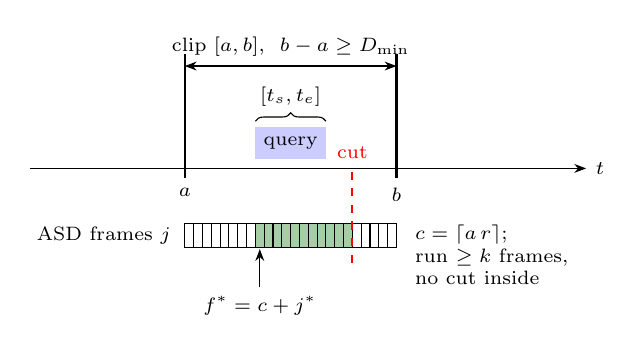
\begin{tikzpicture}[x=0.56cm,y=0.5cm,font=\scriptsize]
\draw[-{Stealth[length=1.5mm]}] (0,0) -- (12.6,0) node[right]{$t$};
\fill[blue!20] (5.1,0.25) rectangle (6.7,1.05);
\node at (5.9,0.65) {query};
\draw[decorate,decoration={brace,amplitude=3pt}] (5.1,1.2) -- (6.7,1.2) node[midway,above=2pt]{$[t_s,t_e]$};
\draw[thick] (3.5,-0.25) -- (3.5,2.9);
\draw[thick] (8.3,-0.25) -- (8.3,2.9);
\draw[{Stealth[length=1.5mm]}-{Stealth[length=1.5mm]}] (3.5,2.6) -- (8.3,2.6) node[midway,above]{clip $[a,b]$, \ $b-a\ge D_{\min}$};
\node[below] at (3.5,-0.25) {$a$};
\node[below] at (8.3,-0.25) {$b$};
\foreach \i in {8,...,18} {\fill[green!45!black!35] (3.5+0.2*\i,-2.0) rectangle (3.7+0.2*\i,-1.4);}
\foreach \i in {0,...,23} {\draw (3.5+0.2*\i,-2.0) rectangle (3.7+0.2*\i,-1.4);}
\node[left] at (3.4,-1.7) {ASD frames $j$};
\draw[red,dashed,thick] (7.3,-2.4) -- (7.3,0.0);
\node[red,above] at (7.3,0.0) {cut};
\draw[-{Stealth[length=1.5mm]}] (5.2,-3.0) -- (5.2,-2.05);
\node[below] at (5.2,-3.0) {$f^\ast=c+j^\ast$};
\node[anchor=north west,align=left] at (8.5,-1.2) {$c=\lceil a\,r\rceil$;\\run $\ge k$ frames,\\no cut inside};
\end{tikzpicture}
\caption{Candidate window and frame selection. The matched span is padded and widened to at least $D_{\min}$. Shaded cells are frames in which the face associated with the query speaker is speaking. The run ends at a shot cut, and its first frame, offset by $c$, is reported.}
\label{fig:window}
\end{figure}

\subsection{Confidence and Outcome}
A selected frame is scored with a weighted mean of terms $x_i\in[0,1]$:
\begin{equation}
C=\frac{\sum_{i\in A} w_i\,x_i}{\sum_{i\in A} w_i}.
\label{eq:conf}
\end{equation}
The four terms are the match score $\rho/100$, the mean recognizer probability of the matched words, the mean face-detection confidence over the run, and a stability term $\min(1, L/2k)$ for a run of $L$ frames, which saturates at twice the minimum length. Their weights are 0.40, 0.25, 0.25 and 0.10. In discovery mode the active set $A$ leaves out the match term. Scoring that term as 1.0 instead would give every discovery result 0.40 for a comparison that never took place, and identical visual evidence would then clear a lower bar in one mode than in the other.

Results with $C\ge0.70$ are reported as \textit{success}, results with $0.45\le C<0.70$ as \textit{ambiguous} with the weakest term named, and lower scores as \textit{not on screen}. Three conditions override a high score and force \textit{ambiguous}: no diarized speaker was available for the line, so any speaking face was accepted; a frame reached the service's limit of five faces, so faces may have been dropped; or two faces were speaking at the same time.

\subsection{Target and Discovery Modes}
Algorithm~\ref{alg:modea} gives the target-mode procedure. Candidates are verified in chronological order and the loop stops at the first one that qualifies. This bounds the cost, and it also guarantees that an earlier on-screen occurrence is never displaced by a later one that happened to be checked first. A detection failure on one candidate is recorded and the loop moves on. Discovery mode runs the same verification on every candidate, files each result into one of three lists, and accepts optional limits on candidate count or wall-clock time. A sweep stopped by a limit is marked as truncated and reports how many candidates were processed out of the total. A guard raises an error only if every window in a run of three or more comes back with no speaker association at all, the signature of diarization never reaching the service. A single such window is the ordinary off-camera case and is reported as an answer, not as a fault.

\begin{algorithm}[t]
\caption{Target-mode localization}
\label{alg:modea}
\small
\begin{algorithmic}[1]
\Require video $V$, query $q$
\Ensure frame $f^\ast$ with time and confidence, or a reasoned negative answer
\State $M \gets \textsc{NormalizeCFR}(V)$;\ \ $r \gets M.\mathit{fps}$
\State $\mathcal{W} \gets \textsc{Align}(\textsc{ASR}(M.a),\ \textsc{Diarize}(M.a))$
\State $\mathcal{Q} \gets \textsc{Match}(\mathcal{W}, q, \theta_m, \delta)$ \Comment{time order}
\If{$\mathcal{Q}=\emptyset$}
  \State \Return \textit{not found}
\EndIf
\State $\mathcal{E} \gets \emptyset$
\For{each match $m \in \mathcal{Q}$}
  \State $[a,b] \gets \textsc{Window}(m, p, D_{\min}, D_{\max})$
  \State $(\mathit{clip}, c) \gets \textsc{Trim}(M.v, a, b)$
  \State $R \gets \textsc{ASD}(\mathit{clip}, \textsc{Diar}(\mathcal{W}\cap[a,b]))$
  \State $h \gets \textsc{Select}(R, \sigma_m, k, \textsc{Cuts}(\mathit{clip}))$
  \If{$h$ is a qualifying run}
    \State $f^\ast \gets c + h.j$
    \State \Return $\bigl(f^\ast,\ f^\ast/r,\ \textsc{Confidence}(m,h)\bigr)$
  \EndIf
  \State $\mathcal{E} \gets \mathcal{E}\cup\{h.\mathit{reason}\}$
\EndFor
\State \Return \textit{not on screen} with the most informative reason in $\mathcal{E}$
\end{algorithmic}
\end{algorithm}

% ---------------------------------------------------------------------------
\section{Implementation}
\label{sec:impl}

The system is written in Python~3.11, roughly ten thousand lines excluding vendored client code, and follows a ports-and-adapters structure. The orchestrator depends only on abstract interfaces for the video source, transcriber, diarizer, ASD provider, frame extractor and cache. A single composition module binds the concrete implementations, so replacing the hosted ASD backend with a local model such as Light-ASD~\cite{liao2023lightasd} touches no pipeline code; a placeholder provider for that model is already registered behind the same interface. Heavy libraries are imported lazily, so a health check or a rejected URL never loads several gigabytes of model weights.

Every stage raises a typed error that names the stage and suggests a remedy. The orchestrator also catches unforeseen exceptions and returns a structured result naming the stage that was running, without forwarding tracebacks that could expose file paths or credentials. Three caches are kept on disk: the downloaded and normalized media as a pair, keyed by the canonicalized URL; transcripts, keyed by audio hash, model and quantization; and diarization output. Including quantization in the key is necessary: the same audio produced 325 words with int8 weights on the CPU and 337 with int8/float16 weights on the GPU.

The pipeline is exposed in three ways. A command-line tool uses distinct exit codes for ``frame found'', ``pipeline answered no'' and ``pipeline failed''. An HTTP API built with FastAPI accepts a job, returns immediately and is polled for stage-level progress. A React web interface is served by the same process. The code base includes more than one thousand unit and integration tests. Table~\ref{tab:params} lists the operating parameters, and Fig.~\ref{fig:arch} shows the complete control flow, including validation and error paths.

\begin{table}[t]
\centering
\caption{Operating parameters}
\label{tab:params}
\footnotesize
\begin{tabular}{@{}llp{3.3cm}@{}}
\toprule
Parameter & Value & Purpose \\
\midrule
$\theta_m$ & 70 & minimum match score $\rho$ \\
$\delta$ & 2 tokens & window length slack \\
$p$ & 1.5\,s & padding for timestamp jitter \\
$D_{\min}$ / $D_{\max}$ & 3.5\,s / 30\,s & clip length bounds \\
$\tau$ & 120\,ms & minimum speaking run \\
Scene threshold & 0.4 & shot-cut detection \\
Face limit & 5 & per-frame cap of the ASD service \\
Min.\ turn / gap & 0.25\,s / 0.75\,s & diarization clean-up, segment split \\
Weights & .40/.25/.25/.10 & match / ASR / face / stability \\
Bands & 0.70 / 0.45 & success / ambiguous thresholds \\
Decoding & beam 5, $T{=}0$ & deterministic Whisper output \\
Clip height & 720 lines & ASD upload size \\
\bottomrule
\end{tabular}
\end{table}

\begin{figure*}[t]
\centering
\includegraphics[height=0.42\textheight,keepaspectratio]{figures/architecture.png}
\caption{Detailed control flow of the implemented system: media validation, the two operating modes, the per-candidate verification loop and the error paths. Every terminal path produces a structured JSON result.}
\label{fig:arch}
\end{figure*}

% ---------------------------------------------------------------------------
\section{Experimental Setup}
\label{sec:setup}

The experiments use a publicly available 610\,s excerpt from a feature film, at 1080p and 23.976 frames/s. It contains several characters, frequent shot changes, both close-ups and wide shots, and a long fight sequence narrated as internal monologue, which provides natural voice-over material. Transcription and diarization ran on a laptop with an NVIDIA RTX~4060 GPU, using Whisper large-v3 with int8/float16 weights. Active speaker detection used the hosted NVIDIA service.

No public benchmark annotates frames for this task, so we report four kinds of evidence instead of accuracy against ground truth: (i) per-stage latency for a first run and a repeated run; (ii) the share of footage sent for visual analysis; (iii) run-to-run determinism; and (iv) the distribution of discovery outcomes, with every off-camera decision checked against the film. The target-mode query was ``Yes, and you, sir, an excellent policeman.'' Each frame the system returned was opened and inspected by hand.

% ---------------------------------------------------------------------------
\section{Results}
\label{sec:results}

\subsection{Target Mode}
The query matched one transcript span, which alignment attributed to diarized speaker SPEAKER\_03. A single 4\,s window was verified, and the selector returned frame 983 at 00:00:40.999 with status \textit{success} and confidence 0.929. The extracted image shows the speaking character on camera, mid-line. Because only the matched window is processed visually, 0.7\% of the footage reached the ASD service. The same query on a feature-length film would still cost one request, since the visual cost grows with the number of matches, not with duration.

Table~\ref{tab:latency} breaks down the latency. A first run took about 145\,s, dominated by the forced-CFR re-encode (about 100\,s) and transcription (37\,s). A repeated query on the same video took about 15\,s, because acquisition, normalization, transcription and diarization were served from the cache, leaving essentially the detection request. For a library that is searched repeatedly, the expensive work is therefore paid once per asset rather than once per query.

\begin{table}[t]
\centering
\caption{Stage latency on the 610\,s test video (target mode)}
\label{tab:latency}
\footnotesize
\begin{tabular}{@{}lrr@{}}
\toprule
Stage & First run (s) & Repeat run (s) \\
\midrule
Acquisition & $\approx$5 & 0 (cached) \\
CFR normalization & $\approx$100 & 0 (cached) \\
Transcription & 37 & 7 \\
Diarization & 19 & $<$1 \\
Alignment and matching & $<$1 & $<$1 \\
ASD, per candidate & 2.4--8.5 & 2.4--8.5 \\
\midrule
End to end & $\approx$145 & $\approx$15 \\
\bottomrule
\end{tabular}
\end{table}

\subsection{Discovery Mode}
Without a query, the pipeline built 31 candidates and processed all of them. Nine were classified as on screen, five as ambiguous and seventeen as not on screen (Table~\ref{tab:modes}). The off-camera group was not scattered across the video. Seven consecutive utterances between 07:18 and 08:13 were all rejected, and they coincide exactly with the internal-monologue fight sequence, during which the narrating character's mouth does not move. A caption or transcript search would have returned each of those seven lines as a hit. Detection requests took between 2.4\,s and 8.5\,s each, and the sweep sent about 28\% of the footage for visual analysis.

\begin{table}[t]
\centering
\caption{Cost and output of the two operating modes}
\label{tab:modes}
\footnotesize
\begin{tabular}{@{}lcc@{}}
\toprule
Quantity & Target & Discovery \\
\midrule
ASD requests & 1 & 31 \\
Footage analysed visually & 0.7\% & $\approx$28\% \\
Result & 1 frame & 9 / 5 / 17 lines$^\dagger$ \\
Time with cached preprocessing & $\approx$15\,s & $\approx$90\,s \\
\bottomrule
\end{tabular}

\vspace{2pt}
\parbox{\columnwidth}{\scriptsize $^\dagger$on screen / ambiguous / not on screen.}
\end{table}

\subsection{Determinism}
Three consecutive runs returned the same frame indices (144, 535, 750, 869, 944, 983 and 1220) with confidences identical to three decimal places. This follows from the pinned decoding settings, from deterministic tie-breaking in alignment and matching, and from expressing every threshold in physical units derived from the measured frame rate.

\subsection{Minimum Clip Length of the ASD Service}
\label{sec:probe}
The service accepts arbitrarily short clips without complaint. To find out what it does with them, a window known to contain a visible speaker was trimmed to lengths between 0.12\,s and 4.90\,s. Every clip of 2.90\,s or less returned zero frames, whereas 3.00\,s returned 72 frames and 4.90\,s returned 118 (Fig.~\ref{fig:probe}). Seventy-two frames is exactly three seconds at that clip's rate, which points to a fixed internal context window rather than an explicit length check. An empty response cannot be told apart from ``no one is on screen'', so short windows would be misclassified silently. In an early discovery run, 23 of 37 candidates were shorter than this floor. Padding such windows to 3.5\,s (Section~\ref{sec:cand}) instead of discarding them keeps one-word lines such as ``Yes.'' verifiable.

\begin{figure}[t]
\centering
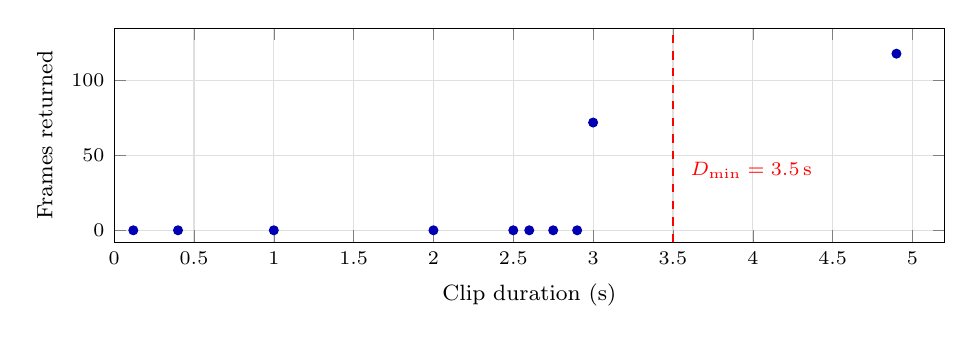
\begin{tikzpicture}
\begin{axis}[
  width=\columnwidth, height=4.3cm,
  xlabel={Clip duration (s)}, ylabel={Frames returned},
  xmin=0, xmax=5.2, ymin=-8, ymax=135,
  grid=major, grid style={gray!25},
  tick label style={font=\scriptsize}, label style={font=\footnotesize}
]
\addplot[only marks, mark=*, mark size=1.6pt, blue!70!black]
  coordinates {(0.12,0) (0.40,0) (1.00,0) (2.00,0) (2.50,0) (2.60,0) (2.75,0) (2.90,0) (3.00,72) (4.90,118)};
\addplot[dashed, red, thick] coordinates {(3.5,-8) (3.5,135)};
\node[font=\scriptsize, anchor=west, red] at (axis cs:3.55,40) {$D_{\min}=3.5$\,s};
\end{axis}
\end{tikzpicture}
\caption{Frames returned by the hosted ASD service for clips of increasing length cut from the same shot of a visible speaker. Below about 3\,s the service returns nothing, which motivates the floor $D_{\min}$.}
\label{fig:probe}
\end{figure}

% ---------------------------------------------------------------------------
\section{Discussion and Limitations}
\label{sec:discussion}

The results support a claim that is partly qualitative. Separating on-camera delivery from off-camera speech is feasible with existing pretrained components, provided the composition enforces speaker consistency and treats per-frame detector output with care. Several failure modes of the hosted detector (short clips, late diarization, a misread sentinel value) produce plausible wrong answers rather than errors. Each was found only by running the system on real footage, and each is now checked explicitly in code and covered by tests.

The evaluation has clear limits. It is a case study on a single video. There is no frame-level ground truth, and the three output groups were checked by inspection rather than scored against independent annotations, so the precision and recall of the on-screen decision, and the error of $f^\ast$ in frames, remain to be measured. The selector returns the start of the earliest qualifying run anywhere in the padded window. If the same speaker is already talking just before the queried words, that run can begin slightly before the phrase itself; restricting selection to frames after the match onset is a straightforward refinement. The approach also inherits the weaknesses of its parts: recognition errors on noisy audio, diarization confusion in crowded scenes, and the detector's limit of five faces per frame, which makes crowd shots ambiguous by construction. The default detector is a hosted service, so results depend on network access and on a model that cannot be inspected. Finally, the system assumes English, the primary audio track and one video per request. The API currently runs jobs in-process without isolating their working directories, so concurrent jobs must be serialized by the client.

% ---------------------------------------------------------------------------
\section{Conclusion and Future Work}
\label{sec:conclusion}

We presented a query-driven pipeline that returns the first frame in which a given line of dialogue is spoken by a visible speaker, or lists every on-screen line when no query is given. It verifies speech visually only where the transcript places the line, requires the face found speaking to belong to the diarized speaker of the queried words, and reports an explained confidence instead of a bare decision. On a 610\,s film excerpt it localized the target line with one detection request covering 0.7\% of the footage, answered repeated queries in about 15\,s, and ruled an entire internal-monologue scene off camera without being told that the scene existed.

Future work will build a benchmark with frame-level on-screen and off-screen labels across films, television and interviews. That benchmark will measure localization error and the precision of the off-camera decision against a caption-search baseline and against the character-aware subtitling system of~\cite{huh2024context}. We also plan to replace the hosted detector with a local model trained for robustness~\cite{liao2025lrasd,nguyen2026unitalk}, to use speaker enrolment~\cite{wang2026beyond} to name characters, and to support further languages and audio tracks.

\section*{Acknowledgment}
The authors used an AI assistant (Claude, Anthropic) during software development and to help draft and edit parts of this manuscript. All technical content, measurements and citations were reviewed and verified by the authors, who take full responsibility for the paper.

\bibliographystyle{IEEEtran}
\bibliography{refs}

\end{document}
